% Options for packages loaded elsewhere
\PassOptionsToPackage{unicode}{hyperref}
\PassOptionsToPackage{hyphens}{url}
\PassOptionsToPackage{dvipsnames,svgnames,x11names}{xcolor}
%
\documentclass[
  authoryear,
  preprint,
  3p]{elsarticle}

\usepackage{amsmath,amssymb}
\usepackage{iftex}
\ifPDFTeX
  \usepackage[T1]{fontenc}
  \usepackage[utf8]{inputenc}
  \usepackage{textcomp} % provide euro and other symbols
\else % if luatex or xetex
  \usepackage{unicode-math}
  \defaultfontfeatures{Scale=MatchLowercase}
  \defaultfontfeatures[\rmfamily]{Ligatures=TeX,Scale=1}
\fi
\usepackage{lmodern}
\ifPDFTeX\else  
    % xetex/luatex font selection
\fi
% Use upquote if available, for straight quotes in verbatim environments
\IfFileExists{upquote.sty}{\usepackage{upquote}}{}
\IfFileExists{microtype.sty}{% use microtype if available
  \usepackage[]{microtype}
  \UseMicrotypeSet[protrusion]{basicmath} % disable protrusion for tt fonts
}{}
\makeatletter
\@ifundefined{KOMAClassName}{% if non-KOMA class
  \IfFileExists{parskip.sty}{%
    \usepackage{parskip}
  }{% else
    \setlength{\parindent}{0pt}
    \setlength{\parskip}{6pt plus 2pt minus 1pt}}
}{% if KOMA class
  \KOMAoptions{parskip=half}}
\makeatother
\usepackage{xcolor}
\setlength{\emergencystretch}{3em} % prevent overfull lines
\setcounter{secnumdepth}{5}
% Make \paragraph and \subparagraph free-standing
\makeatletter
\ifx\paragraph\undefined\else
  \let\oldparagraph\paragraph
  \renewcommand{\paragraph}{
    \@ifstar
      \xxxParagraphStar
      \xxxParagraphNoStar
  }
  \newcommand{\xxxParagraphStar}[1]{\oldparagraph*{#1}\mbox{}}
  \newcommand{\xxxParagraphNoStar}[1]{\oldparagraph{#1}\mbox{}}
\fi
\ifx\subparagraph\undefined\else
  \let\oldsubparagraph\subparagraph
  \renewcommand{\subparagraph}{
    \@ifstar
      \xxxSubParagraphStar
      \xxxSubParagraphNoStar
  }
  \newcommand{\xxxSubParagraphStar}[1]{\oldsubparagraph*{#1}\mbox{}}
  \newcommand{\xxxSubParagraphNoStar}[1]{\oldsubparagraph{#1}\mbox{}}
\fi
\makeatother

\usepackage{color}
\usepackage{fancyvrb}
\newcommand{\VerbBar}{|}
\newcommand{\VERB}{\Verb[commandchars=\\\{\}]}
\DefineVerbatimEnvironment{Highlighting}{Verbatim}{commandchars=\\\{\}}
% Add ',fontsize=\small' for more characters per line
\usepackage{framed}
\definecolor{shadecolor}{RGB}{241,243,245}
\newenvironment{Shaded}{\begin{snugshade}}{\end{snugshade}}
\newcommand{\AlertTok}[1]{\textcolor[rgb]{0.68,0.00,0.00}{#1}}
\newcommand{\AnnotationTok}[1]{\textcolor[rgb]{0.37,0.37,0.37}{#1}}
\newcommand{\AttributeTok}[1]{\textcolor[rgb]{0.40,0.45,0.13}{#1}}
\newcommand{\BaseNTok}[1]{\textcolor[rgb]{0.68,0.00,0.00}{#1}}
\newcommand{\BuiltInTok}[1]{\textcolor[rgb]{0.00,0.23,0.31}{#1}}
\newcommand{\CharTok}[1]{\textcolor[rgb]{0.13,0.47,0.30}{#1}}
\newcommand{\CommentTok}[1]{\textcolor[rgb]{0.37,0.37,0.37}{#1}}
\newcommand{\CommentVarTok}[1]{\textcolor[rgb]{0.37,0.37,0.37}{\textit{#1}}}
\newcommand{\ConstantTok}[1]{\textcolor[rgb]{0.56,0.35,0.01}{#1}}
\newcommand{\ControlFlowTok}[1]{\textcolor[rgb]{0.00,0.23,0.31}{\textbf{#1}}}
\newcommand{\DataTypeTok}[1]{\textcolor[rgb]{0.68,0.00,0.00}{#1}}
\newcommand{\DecValTok}[1]{\textcolor[rgb]{0.68,0.00,0.00}{#1}}
\newcommand{\DocumentationTok}[1]{\textcolor[rgb]{0.37,0.37,0.37}{\textit{#1}}}
\newcommand{\ErrorTok}[1]{\textcolor[rgb]{0.68,0.00,0.00}{#1}}
\newcommand{\ExtensionTok}[1]{\textcolor[rgb]{0.00,0.23,0.31}{#1}}
\newcommand{\FloatTok}[1]{\textcolor[rgb]{0.68,0.00,0.00}{#1}}
\newcommand{\FunctionTok}[1]{\textcolor[rgb]{0.28,0.35,0.67}{#1}}
\newcommand{\ImportTok}[1]{\textcolor[rgb]{0.00,0.46,0.62}{#1}}
\newcommand{\InformationTok}[1]{\textcolor[rgb]{0.37,0.37,0.37}{#1}}
\newcommand{\KeywordTok}[1]{\textcolor[rgb]{0.00,0.23,0.31}{\textbf{#1}}}
\newcommand{\NormalTok}[1]{\textcolor[rgb]{0.00,0.23,0.31}{#1}}
\newcommand{\OperatorTok}[1]{\textcolor[rgb]{0.37,0.37,0.37}{#1}}
\newcommand{\OtherTok}[1]{\textcolor[rgb]{0.00,0.23,0.31}{#1}}
\newcommand{\PreprocessorTok}[1]{\textcolor[rgb]{0.68,0.00,0.00}{#1}}
\newcommand{\RegionMarkerTok}[1]{\textcolor[rgb]{0.00,0.23,0.31}{#1}}
\newcommand{\SpecialCharTok}[1]{\textcolor[rgb]{0.37,0.37,0.37}{#1}}
\newcommand{\SpecialStringTok}[1]{\textcolor[rgb]{0.13,0.47,0.30}{#1}}
\newcommand{\StringTok}[1]{\textcolor[rgb]{0.13,0.47,0.30}{#1}}
\newcommand{\VariableTok}[1]{\textcolor[rgb]{0.07,0.07,0.07}{#1}}
\newcommand{\VerbatimStringTok}[1]{\textcolor[rgb]{0.13,0.47,0.30}{#1}}
\newcommand{\WarningTok}[1]{\textcolor[rgb]{0.37,0.37,0.37}{\textit{#1}}}

\providecommand{\tightlist}{%
  \setlength{\itemsep}{0pt}\setlength{\parskip}{0pt}}\usepackage{longtable,booktabs,array}
\usepackage{calc} % for calculating minipage widths
% Correct order of tables after \paragraph or \subparagraph
\usepackage{etoolbox}
\makeatletter
\patchcmd\longtable{\par}{\if@noskipsec\mbox{}\fi\par}{}{}
\makeatother
% Allow footnotes in longtable head/foot
\IfFileExists{footnotehyper.sty}{\usepackage{footnotehyper}}{\usepackage{footnote}}
\makesavenoteenv{longtable}
\usepackage{graphicx}
\makeatletter
\def\maxwidth{\ifdim\Gin@nat@width>\linewidth\linewidth\else\Gin@nat@width\fi}
\def\maxheight{\ifdim\Gin@nat@height>\textheight\textheight\else\Gin@nat@height\fi}
\makeatother
% Scale images if necessary, so that they will not overflow the page
% margins by default, and it is still possible to overwrite the defaults
% using explicit options in \includegraphics[width, height, ...]{}
\setkeys{Gin}{width=\maxwidth,height=\maxheight,keepaspectratio}
% Set default figure placement to htbp
\makeatletter
\def\fps@figure{htbp}
\makeatother

\makeatletter
\@ifpackageloaded{caption}{}{\usepackage{caption}}
\AtBeginDocument{%
\ifdefined\contentsname
  \renewcommand*\contentsname{Table of contents}
\else
  \newcommand\contentsname{Table of contents}
\fi
\ifdefined\listfigurename
  \renewcommand*\listfigurename{List of Figures}
\else
  \newcommand\listfigurename{List of Figures}
\fi
\ifdefined\listtablename
  \renewcommand*\listtablename{List of Tables}
\else
  \newcommand\listtablename{List of Tables}
\fi
\ifdefined\figurename
  \renewcommand*\figurename{Figure}
\else
  \newcommand\figurename{Figure}
\fi
\ifdefined\tablename
  \renewcommand*\tablename{Table}
\else
  \newcommand\tablename{Table}
\fi
}
\@ifpackageloaded{float}{}{\usepackage{float}}
\floatstyle{ruled}
\@ifundefined{c@chapter}{\newfloat{codelisting}{h}{lop}}{\newfloat{codelisting}{h}{lop}[chapter]}
\floatname{codelisting}{Listing}
\newcommand*\listoflistings{\listof{codelisting}{List of Listings}}
\makeatother
\makeatletter
\makeatother
\makeatletter
\@ifpackageloaded{caption}{}{\usepackage{caption}}
\@ifpackageloaded{subcaption}{}{\usepackage{subcaption}}
\makeatother
\journal{Journal Name}

\ifLuaTeX
  \usepackage{selnolig}  % disable illegal ligatures
\fi
\usepackage[]{natbib}
\bibliographystyle{elsarticle-harv}
\usepackage{bookmark}

\IfFileExists{xurl.sty}{\usepackage{xurl}}{} % add URL line breaks if available
\urlstyle{same} % disable monospaced font for URLs
\hypersetup{
  pdftitle={A tutorial of Bayesian beta regressions with brms in R},
  pdfauthor={Stefano Coretta},
  pdfkeywords={keyword1, keyword2},
  colorlinks=true,
  linkcolor={blue},
  filecolor={Maroon},
  citecolor={Blue},
  urlcolor={Blue},
  pdfcreator={LaTeX via pandoc}}


\setlength{\parindent}{6pt}
\begin{document}

\begin{frontmatter}
\title{A tutorial of Bayesian beta regressions with brms in R}
\author[1]{Stefano Coretta%
\corref{cor1}%
\fnref{fn1}}
 \ead{s.coretta@ed.ac.uk} 

\affiliation[1]{organization={University of Edinburgh, Linguistics and
English Language},addressline={3 George
Sq},city={Edinburgh},postcode={EH8 9AD},postcodesep={}}

\cortext[cor1]{Corresponding author}
\fntext[fn1]{This is the first author footnote.}
        
\begin{abstract}
This is the abstract. Lorem ipsum dolor sit amet, consectetur adipiscing
elit. Vestibulum augue turpis, dictum non malesuada a, volutpat eget
velit. Nam placerat turpis purus, eu tristique ex tincidunt et. Mauris
sed augue eget turpis ultrices tincidunt. Sed et mi in leo porta
egestas. Aliquam non laoreet velit. Nunc quis ex vitae eros aliquet
auctor nec ac libero. Duis laoreet sapien eu mi luctus, in bibendum leo
molestie. Sed hendrerit diam diam, ac dapibus nisl volutpat vitae.
Aliquam bibendum varius libero, eu efficitur justo rutrum at. Sed at
tempus elit.
\end{abstract}





\begin{keyword}
    keyword1 \sep 
    keyword2
\end{keyword}
\end{frontmatter}
    

\section{Introduction}\label{introduction}

Phonetic research often involves numeric continuous outcome variables,
like durations, frequencies, loudness and ratios. Another commonly
employed type of outcome variable are proportions: for example,
proportion of voicing during closure, vocal folds contact quotient,
gesture amplitude, nasalance. Moreover, virtually any measure can be
MIN-MAX normalised, a procedure which transforms values so that they are
in the range 0--1.

Regression models are very common, but there is a tendency of using
Gaussian distribution families (i.e.~probability distributions for the
outcome variable) for anything that is numeric. A possible reason is
that the base R function for fitting regression models, \texttt{lm()},
and the lme4 function used to fit regression models with varying terms,
\texttt{lmer()}, both fit Gaussian regressions by default and the user
does not have to specify the distribution family. This tacit defaulting
to Gaussian models is also reflected in teaching practices, where test
and models using the Gaussian distribution are the first to be taught,
due to their relative simplicity and the fact that other models are
generalisations of Gaussian models.

However, proportion are naturally not Gaussian, since they are limited
between 0 and 1. The theoretical distribution that generates values with
this characteristics is the beta distribution. Thus, regression models
with proportions as the outcome variable should be fitted using a beta
distribution as the distribution family. This tutorial introduces
researchers to beta regression models in R using the package brms.
Familiarity with regression modelling in R with a package like lme4 is
assumed, but no prior knowledge of Bayesian statistics is necessary.

\section{The beta distribution}\label{the-beta-distribution}

\ldots{}

\section{Case study 1: voicing within consonant
closure}\label{case-study-1-voicing-within-consonant-closure}

For the first case study, we will model the proportion of voicing within
consonant closure. The measurements come from a data set of audio and
electroglottographic (EGG) recordings of 19 speakers of Northwestern
Italian. The participants read frame sentences which included target
words of the form /CVCo/, where /C/ was either /k, t, p/ in all
permutations and /V/ was either /i, e, a, ɔ, u/ (two resulting words,
/peto/ and /kako/ were excluded because they are profanities), for a
total of 43 target words. There were 4 different frame sentence, with a
total of 172 trials per participant (3,268 grand total). The actual
observation count is 2,419, after removing speech errors, EGG
measurement errors, and cases in which voicing ceased before the closure
onset/after the closure offset of the second /C/.

The proportion of voicing during the closure of the second /C/ was
calculated as the proportion of contiguous voicing duration after
closure onset to total duration of closure. The following code chunk
attaches the tidyverse packages (for reading and wrangling data) and
loads the \texttt{ita\_egg} tibble (data frame). The tibble is filtered
so as to remove voicing proportions (\texttt{voi\_clo\_prop}) that are
smaller than 0 and greater than 1. The variables \texttt{vowel} and
\texttt{c2} are converted to factors to specify the order of the levels.

\begin{Shaded}
\begin{Highlighting}[]
\CommentTok{\# attach tidyverse and set light theme for plots}
\FunctionTok{library}\NormalTok{(tidyverse)}
\FunctionTok{theme\_set}\NormalTok{(}\FunctionTok{theme\_light}\NormalTok{())}

\CommentTok{\# load tibble}
\FunctionTok{load}\NormalTok{(}\StringTok{"data/coretta2018/ita\_egg.rda"}\NormalTok{)}

\CommentTok{\# filter and mutate data}
\NormalTok{ita\_egg }\OtherTok{\textless{}{-}}\NormalTok{ ita\_egg }\SpecialCharTok{|\textgreater{}} 
  \FunctionTok{filter}\NormalTok{(voi\_clo\_prop }\SpecialCharTok{\textgreater{}} \DecValTok{0}\NormalTok{, voi\_clo\_prop }\SpecialCharTok{\textless{}} \DecValTok{1}\NormalTok{) }\SpecialCharTok{|\textgreater{}} 
  \FunctionTok{mutate}\NormalTok{(}
    \AttributeTok{vowel =} \FunctionTok{factor}\NormalTok{(vowel, }\AttributeTok{levels =} \FunctionTok{c}\NormalTok{(}\StringTok{"i"}\NormalTok{, }\StringTok{"e"}\NormalTok{, }\StringTok{"a"}\NormalTok{, }\StringTok{"o"}\NormalTok{, }\StringTok{"u"}\NormalTok{)),}
    \AttributeTok{c2 =} \FunctionTok{factor}\NormalTok{(c2, }\AttributeTok{levels =} \FunctionTok{c}\NormalTok{(}\StringTok{"k"}\NormalTok{, }\StringTok{"t"}\NormalTok{, }\StringTok{"p"}\NormalTok{))}
\NormalTok{  )}
\end{Highlighting}
\end{Shaded}

Here is what the tibble looks like.

\begin{Shaded}
\begin{Highlighting}[]
\NormalTok{ita\_egg}
\end{Highlighting}
\end{Shaded}

\begin{verbatim}
# A tibble: 2,419 x 53
   speaker ipu    stimulus    sentence_ons sentence_off word_ons word_off v1_ons
   <chr>   <chr>  <chr>              <dbl>        <dbl>    <dbl>    <dbl>  <dbl>
 1 it01    ipu_1  Ripete 'po~         13.2         14.9     13.7     14.1   13.9
 2 it01    ipu_2  Ripete 'to~         16.9         18.6     17.4     17.9   17.5
 3 it01    ipu_3  Ripete 'pa~         20.2         21.9     20.7     21.1   20.8
 4 it01    ipu_4  Sentivo 't~         23.5         25.1     24.0     24.4   24.1
 5 it01    ipu_5  Sentivo 't~         26.3         27.8     26.8     27.2   26.9
 6 it01    ipu_6  Scrivete '~         29.2         30.9     29.7     30.1   29.8
 7 it01    ipu_7  Sentivo 'c~         32.1         33.6     32.6     33.1   32.8
 8 it01    ipu_8  Scrivete '~         35.0         36.6     35.5     35.9   35.6
 9 it01    ipu_9  Ha detto '~         41.9         43.5     42.3     42.7   42.4
10 it01    ipu_10 Sentivo 'p~         47.4         48.9     47.9     48.4   48.1
# i 2,409 more rows
# i 45 more variables: c2_ons <dbl>, v2_ons <dbl>, voice_ons <dbl>,
#   voice_off <dbl>, c1_rel <dbl>, c2_rel <dbl>, stimulus_id <dbl>,
#   sentence <chr>, word <chr>, c1 <chr>, vowel <fct>, c2 <fct>,
#   backness <chr>, height <fct>, c1_place <fct>, c2_place <fct>,
#   v1_duration <dbl>, c2_clos_duration <dbl>, rel_voff <dbl>,
#   sent_duration <dbl>, speech_rate <dbl>, speech_rate_c <dbl>, ...
\end{verbatim}

Figure~\ref{fig-ita-egg} shows the raw voicing duration proportion
values split by vowel /i, e, a, ɔ, u/ and second consonant /k, t, p/ in
the /CVCo/ target words. The plot suggests that, on average, the voicing
proportion is slightly lower with /k/ than with /t, p/. Moreover, there
is greater variability between vowels in /t, p/ than in /k/. We will use
a beta regression model to assess these patterns. {[}``expectations''
XXX{]}

\begin{figure}

\centering{

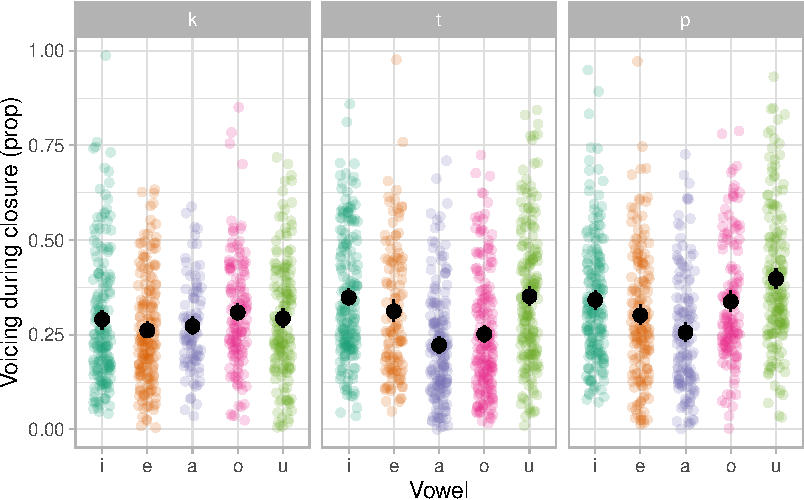
\includegraphics{manuscript_files/figure-pdf/fig-ita-egg-1.pdf}

}

\caption{\label{fig-ita-egg}Proportion of voicing during the closure of
the second consonant in /CVCo/ words by vowel and the second consonant.}

\end{figure}%

We will use brms to fit Bayesian beta regressions. {[}XXX why
Bayesian{]}. The model has voicing proportion as the outcome variable
and the following terms: an interaction between vowel (/i, e, a, ɔ, u/)
and second consonant C2 (/k, t, p/), centred speech rate (number of
syllables per second); as varying (aka random) terms, by-speaker varying
coefficients for the vowel/consonant interaction and for centred speech
rate.\footnote{Footnote about Gelman's terminology for random effects.}
The categorical predictors vowel and C2 are coded using indexing rather
than traditional R contrasts: in R, this corresponds to suppressing the
model's intercept with the \texttt{0\ +} syntax; using indexing instead
of contrasts makes it easier to specify priors. For pedagogical
simplicity, the model will use the default priors, but note that in real
data analyses contexts, priors should be specified by the user. I refer
the readers to XXX.

\begin{Shaded}
\begin{Highlighting}[]
\CommentTok{\# attach brms}
\FunctionTok{library}\NormalTok{(brms)}

\CommentTok{\# fit the model}
\CommentTok{\# Takes 3 minutes on MacBook Pro 2020, M1}
\NormalTok{voi\_prop\_bm }\OtherTok{\textless{}{-}} \FunctionTok{brm}\NormalTok{(}
  \CommentTok{\# model formula}
\NormalTok{  voi\_clo\_prop }\SpecialCharTok{\textasciitilde{}}
    \CommentTok{\# constant terms}
    \DecValTok{0} \SpecialCharTok{+}\NormalTok{ vowel}\SpecialCharTok{:}\NormalTok{c2 }\SpecialCharTok{+}\NormalTok{ speech\_rate\_c }\SpecialCharTok{+}
    \CommentTok{\# varying terms}
\NormalTok{    (}\DecValTok{0} \SpecialCharTok{+}\NormalTok{ vowel}\SpecialCharTok{:}\NormalTok{c2 }\SpecialCharTok{+}\NormalTok{ speech\_rate\_c }\SpecialCharTok{|}\NormalTok{ speaker),}
  \CommentTok{\# uses the beta family for the outcome}
  \AttributeTok{family =}\NormalTok{ Beta,}
  \AttributeTok{data =}\NormalTok{ ita\_egg,}
  \AttributeTok{cores =} \DecValTok{4}\NormalTok{,}
  \AttributeTok{seed =} \DecValTok{3749}\NormalTok{,}
  \AttributeTok{file =} \StringTok{"data/cache/voi\_prop\_bm"}
\NormalTok{)}
\end{Highlighting}
\end{Shaded}

The \texttt{summary()} function prints the full model summary. For
conciseness, we will use the \texttt{fixef()} function which prints the
regression coefficients. The full summary with an explanation of each
part can be found in XXX. For each coefficient in the model,
\texttt{fixef()} prints the name of the coefficient, the mean estimate,
the estimate error and the lower and upper limits of a Bayesian Credible
interval (CrI). Here, we print an 80\% CrI. There is nothing special
about 95\% CrI within Bayesian inference and instead experts recommend
to check and report a variety of CrIs. Bayesian CrIs indicate that at a
certain probability levels the ``true'' estimate lies within that
interval: so, for example, a 90\% CrI {[}A, B{]} indicates that there is
a 90\% probability that the ``true'' estimate is between A and B.
Different probability levels correspond to different levels of
confidence: the higher the probability the higher the confidence (always
conditional on data and model). Obtaining CrIs at different probability
levels allows researchers to make more fine-grained inferential
statements than the frequentist significance dichotomy affords. For
simplicity of exposition, we will use 80\% CrIs in this case study but
we strongly recommend researchers to always obtain CrIs at different
levels of probability and base their inferences on all and not one in
particular. To reiterate, in Bayesian inference, an 80\% CrI indicates
the range of values within which the true estimate falls at 80\%
probability or confidence. We round all values to the nearest 2 digits
for clarity.

\begin{Shaded}
\begin{Highlighting}[]
\FunctionTok{round}\NormalTok{(}
  \FunctionTok{fixef}\NormalTok{(voi\_prop\_bm, }\AttributeTok{prob =} \FunctionTok{c}\NormalTok{(}\FloatTok{0.1}\NormalTok{, }\FloatTok{0.9}\NormalTok{)),}
  \AttributeTok{digits =} \DecValTok{2}
\NormalTok{)}
\end{Highlighting}
\end{Shaded}

\begin{verbatim}
              Estimate Est.Error   Q10   Q90
speech_rate_c     0.08      0.06  0.01  0.15
voweli:c2k       -0.91      0.14 -1.08 -0.74
vowele:c2k       -1.08      0.11 -1.22 -0.94
vowela:c2k       -0.99      0.12 -1.14 -0.84
vowelo:c2k       -0.79      0.14 -0.96 -0.62
vowelu:c2k       -1.00      0.16 -1.20 -0.80
voweli:c2t       -0.66      0.11 -0.79 -0.53
vowele:c2t       -0.84      0.14 -1.02 -0.66
vowela:c2t       -1.43      0.13 -1.60 -1.26
vowelo:c2t       -1.15      0.13 -1.31 -0.99
vowelu:c2t       -0.68      0.12 -0.83 -0.54
voweli:c2p       -0.68      0.11 -0.81 -0.54
vowele:c2p       -0.88      0.15 -1.07 -0.68
vowela:c2p       -1.14      0.13 -1.31 -0.98
vowelo:c2p       -0.66      0.11 -0.80 -0.53
vowelu:c2p       -0.44      0.12 -0.59 -0.28
\end{verbatim}

The coefficients of a beta regression are estimated on the log-odds
scale, as in Bernoulli/binomial (aka logistic) regressions. From the
summary, we see that speech rate (number of syllables per second) has a
positive effect on voicing proportion: the 80\% CrI is between 0.01 and
0.15 log-odds {[}\(\beta\) = 0.8, SD = 0.06{]}. Log-odds can be
converted to odd ratios by exponentiating the value: 0.01-0.15 log odds
correspond to an odd ratio of 1.01 to 1.16, or as percentages, to an
increase of voicing of 1 to 16\% for every increase of one syllable per
second. Since this is an 80\% CrI, we can be 80\% confident that the
true effect of speech rate is between 1-16\% increase of voicing
proportion, conditional on the data and model. Note that transforming
measures this way is appropriate \emph{only} with quantile-based
measures (like CrIs) but not with moments like the mean and standard
deviation: to correctly get mean and SDs in the transformed scale, you
must first extract the posterior draws (see below), convert them and
then take moments such as mean and SD (for a more detailed explanation,
see XXX).

Turning now to the coefficients for vowel and C2, given the indexing
approach of coding these variables the model summary and the output of
\texttt{fixef()} reports the \emph{predictions} in log-odds for each
combination of vowel and C2, rather than differences between levels. The
CrIs of the vowel/C2 coefficients span all negative log-odds values:
these correspond to proportions that are lower than 0.5 (which is 0 in
log-odds). This matches the general trends in the raw data, which we
plotted in Figure~\ref{fig-ita-egg}.

Next, we will plot the predicted proportions of each vowel/C2
combination at mean speech rate (i.e.~centred speech rate = 0) and then
calculate the average pair-wise difference in voicing proportion between
/k, t, p/. Finally, we will assess whether there is greater
between-vowel variability in /t, p/ relative to /k/.

Before being able to plot the predictions, it's important to get
familiar with the so-called posterior draws. {[}Bayesian MCMC XXX{]}.
Posterior draws can be conveniently obtained with the
\texttt{as\_draws\_df()}. For the moment, we will extract only the draws
of the constant regression coefficients (model variables starting with
\texttt{b\_}). To check which coefficients are available in a model, use
\texttt{get\_variables()} from the tidybayes package.
\texttt{as\_draws\_df()} returns a tibble where each column contains the
drawn values of a coefficient. The probability distribution of the drawn
values of each coefficient is the posterior probability distribution of
that coefficient. Note that, due to the indexing coding of vowel and C2,
all coefficient except \texttt{b\_speech\_rate\_c} are \emph{predicted
log-odds} for each vowel/C2 combination (the drawn values for
\texttt{b\_speech\_rate\_c} are drawn \emph{differences} in log-odds for
each unit increase of speech rate). The drawn values are in log-odds,
but we can convert them to proportions with \texttt{plogis()} (we will
do this when plotting below).

\begin{Shaded}
\begin{Highlighting}[]
\CommentTok{\# extract only coefficient variables starting with "b\_"}
\NormalTok{voi\_prop\_bm\_draws }\OtherTok{\textless{}{-}} \FunctionTok{as\_draws\_df}\NormalTok{(voi\_prop\_bm, }\AttributeTok{variable =} \StringTok{"\^{}b\_"}\NormalTok{, }\AttributeTok{regex =} \ConstantTok{TRUE}\NormalTok{)}
\NormalTok{voi\_prop\_bm\_draws}
\end{Highlighting}
\end{Shaded}

\begin{verbatim}
# A draws_df: 1000 iterations, 4 chains, and 16 variables
   b_speech_rate_c b_voweli:c2k b_vowele:c2k b_vowela:c2k b_vowelo:c2k
1            0.159        -0.72        -1.05        -1.12        -1.02
2            0.035        -0.75        -1.39        -1.06        -0.89
3            0.126        -0.85        -0.98        -1.10        -0.64
4            0.064        -0.70        -1.07        -1.05        -0.83
5            0.032        -0.77        -1.18        -0.94        -0.70
6            0.073        -0.85        -1.23        -1.06        -0.77
7            0.101        -0.95        -1.07        -1.14        -0.86
8            0.074        -1.02        -1.07        -1.17        -0.83
9            0.087        -1.04        -1.07        -1.26        -0.79
10           0.092        -1.20        -1.04        -0.92        -0.64
   b_vowelu:c2k b_voweli:c2t b_vowele:c2t
1         -1.05        -0.62        -0.80
2         -1.04        -0.67        -0.99
3         -0.91        -0.66        -0.80
4         -1.07        -0.53        -0.87
5         -1.06        -0.63        -0.87
6         -1.00        -0.69        -0.73
7         -1.22        -0.74        -1.08
8         -1.22        -0.73        -1.04
9         -1.14        -0.66        -0.91
10        -0.84        -0.63        -0.61
# ... with 3990 more draws, and 8 more variables
# ... hidden reserved variables {'.chain', '.iteration', '.draw'}
\end{verbatim}

We can now wrangle this tibble and plot the posterior distributions for
each vowel/C2 combination.

\begin{Shaded}
\begin{Highlighting}[]
\NormalTok{voi\_prop\_bm\_draws\_long }\OtherTok{\textless{}{-}}\NormalTok{ voi\_prop\_bm\_draws }\SpecialCharTok{|\textgreater{}} 
  \CommentTok{\# drop b\_speech\_rate\_c before pivoting}
  \FunctionTok{select}\NormalTok{(}\SpecialCharTok{{-}}\NormalTok{b\_speech\_rate\_c) }\SpecialCharTok{|\textgreater{}} 
  \CommentTok{\# pivot vowel:c2 columns}
  \FunctionTok{pivot\_longer}\NormalTok{(}\StringTok{\textasciigrave{}}\AttributeTok{b\_voweli:c2k}\StringTok{\textasciigrave{}}\SpecialCharTok{:}\StringTok{\textasciigrave{}}\AttributeTok{b\_vowelu:c2p}\StringTok{\textasciigrave{}}\NormalTok{, }\AttributeTok{names\_to =} \StringTok{"coeff"}\NormalTok{) }\SpecialCharTok{|\textgreater{}} 
  \CommentTok{\# separate "coeff" labels into type ("b"), vowel and c2}
  \FunctionTok{separate}\NormalTok{(coeff, }\AttributeTok{into =} \FunctionTok{c}\NormalTok{(}\StringTok{"type"}\NormalTok{, }\StringTok{"vowel"}\NormalTok{, }\StringTok{"c2"}\NormalTok{))}
\end{Highlighting}
\end{Shaded}

\begin{verbatim}
Warning: Dropping 'draws_df' class as required metadata was removed.
\end{verbatim}

\begin{Shaded}
\begin{Highlighting}[]
\NormalTok{voi\_prop\_bm\_draws\_long}
\end{Highlighting}
\end{Shaded}

\begin{verbatim}
# A tibble: 60,000 x 7
   .chain .iteration .draw type  vowel  c2     value
    <int>      <int> <int> <chr> <chr>  <chr>  <dbl>
 1      1          1     1 b     voweli c2k   -0.721
 2      1          1     1 b     vowele c2k   -1.05 
 3      1          1     1 b     vowela c2k   -1.12 
 4      1          1     1 b     vowelo c2k   -1.02 
 5      1          1     1 b     vowelu c2k   -1.05 
 6      1          1     1 b     voweli c2t   -0.625
 7      1          1     1 b     vowele c2t   -0.795
 8      1          1     1 b     vowela c2t   -1.40 
 9      1          1     1 b     vowelo c2t   -1.10 
10      1          1     1 b     vowelu c2t   -0.668
# i 59,990 more rows
\end{verbatim}

For plotting, we can use ggplot2 statistics layers from the ggdist
package. \texttt{stat\_halfeye()} plots the density of the posterior
probability (in grey), its median (point) and CrIs (lines). Let's use 60
and 80\% CrIs and transform the log-odds values to proportions with
\texttt{plogis()}.

\begin{Shaded}
\begin{Highlighting}[]
\CommentTok{\# attach ggdist package}
\FunctionTok{library}\NormalTok{(ggdist)}
\end{Highlighting}
\end{Shaded}

\begin{verbatim}

Attaching package: 'ggdist'
\end{verbatim}

\begin{verbatim}
The following objects are masked from 'package:brms':

    dstudent_t, pstudent_t, qstudent_t, rstudent_t
\end{verbatim}

\begin{Shaded}
\begin{Highlighting}[]
\NormalTok{voi\_prop\_bm\_draws\_long }\SpecialCharTok{|\textgreater{}} 
  \FunctionTok{ggplot}\NormalTok{(}\FunctionTok{aes}\NormalTok{(}\FunctionTok{plogis}\NormalTok{(value), vowel)) }\SpecialCharTok{+}
  \FunctionTok{stat\_halfeye}\NormalTok{(}\AttributeTok{.width =} \FunctionTok{c}\NormalTok{(}\FloatTok{0.6}\NormalTok{, }\FloatTok{0.8}\NormalTok{)) }\SpecialCharTok{+}
  \FunctionTok{facet\_grid}\NormalTok{(}\AttributeTok{rows =} \FunctionTok{vars}\NormalTok{(c2))}
\end{Highlighting}
\end{Shaded}

\begin{figure}[H]

\centering{

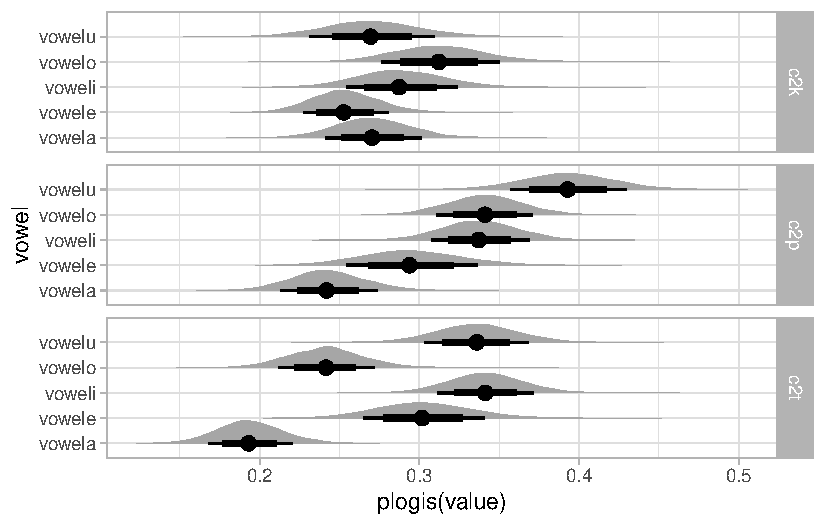
\includegraphics{manuscript_files/figure-pdf/fig-voi-prop-bm-1-1.pdf}

}

\caption{\label{fig-voi-prop-bm-1}}

\end{figure}%

What if we want to plot the average predicted voicing proportion for the
three consonants /k, t, p/? One approach is to take the mean across
vowels within each consonant for each posterior draw, and the posterior
distribution of the resulting list of values is the predicted posterior
distribution of voicing proportion for each consonant, assuming an
``average'' vowel.

\begin{Shaded}
\begin{Highlighting}[]
\NormalTok{voi\_prop\_bm\_draws\_long\_c2 }\OtherTok{\textless{}{-}}\NormalTok{ voi\_prop\_bm\_draws\_long }\SpecialCharTok{|\textgreater{}} 
  \CommentTok{\# grouping by .draw and c2 ensures that averaging applies only within draw and c2}
  \FunctionTok{group\_by}\NormalTok{(.draw, c2) }\SpecialCharTok{|\textgreater{}} 
  \CommentTok{\# calculate the mean value within draw/c2}
  \FunctionTok{summarise}\NormalTok{(}
    \AttributeTok{value\_mean =} \FunctionTok{mean}\NormalTok{(value), }\AttributeTok{.groups =} \StringTok{"drop"}
\NormalTok{  )}

\NormalTok{voi\_prop\_bm\_draws\_long\_c2 }\SpecialCharTok{|\textgreater{}} 
  \FunctionTok{ggplot}\NormalTok{(}\FunctionTok{aes}\NormalTok{(}\FunctionTok{plogis}\NormalTok{(value\_mean), c2)) }\SpecialCharTok{+}
  \FunctionTok{stat\_halfeye}\NormalTok{(}\AttributeTok{.width =} \FunctionTok{c}\NormalTok{(}\FloatTok{0.6}\NormalTok{, }\FloatTok{0.8}\NormalTok{))}
\end{Highlighting}
\end{Shaded}

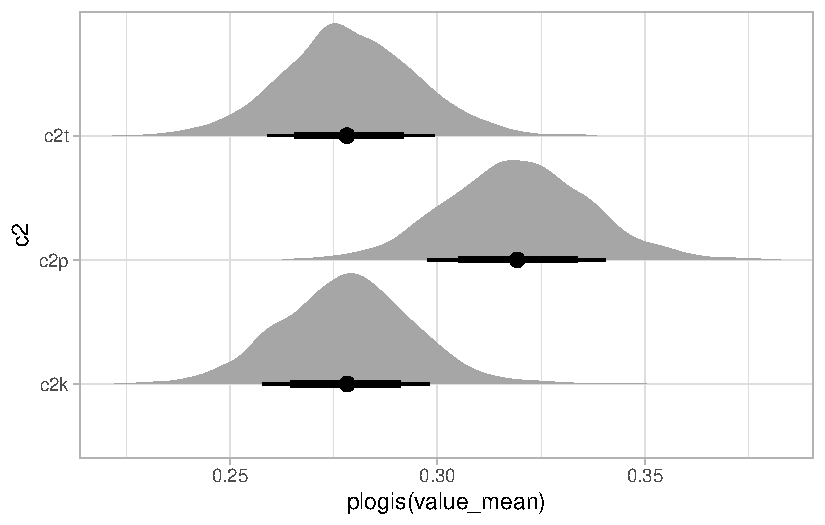
\includegraphics{manuscript_files/figure-pdf/voi-prop-bm-draws-long-c2-1.pdf}

Based on the posterior distributions of the mean voicing proportion by
consonant, /p/ has a somewhat higher voicing proportion than /k/ and
/t/. The real question is: how much higher? We can quantify this by
taking the difference of the drawn values for /p/ and those for /t, k/.
Since we want to compare /t, k/ to /p/, we should first average the
draws of /t, k/ and then take the difference of the averaged draws and
the draws of /p/.

\begin{Shaded}
\begin{Highlighting}[]
\NormalTok{voi\_prop\_bm\_diff }\OtherTok{\textless{}{-}}\NormalTok{ voi\_prop\_bm\_draws\_long\_c2 }\SpecialCharTok{|\textgreater{}} 
  \CommentTok{\# pivot data to create one column per consonant with the mean drawn values,}
  \CommentTok{\# with one draw per raw}
  \FunctionTok{pivot\_wider}\NormalTok{(}\AttributeTok{names\_from =}\NormalTok{ c2, }\AttributeTok{values\_from =}\NormalTok{ value\_mean) }\SpecialCharTok{|\textgreater{}} 
  \FunctionTok{mutate}\NormalTok{(}
    \CommentTok{\# calculate the mean of /k/ and /t/, for each draw}
    \AttributeTok{c2tk =} \FunctionTok{mean}\NormalTok{(}\FunctionTok{c}\NormalTok{(c2k, c2t)),}
    \CommentTok{\# calculate the difference of /p/ and /t, k/}
    \AttributeTok{c2p\_tk\_diff =}\NormalTok{ c2p }\SpecialCharTok{{-}}\NormalTok{ c2tk}
\NormalTok{  )}

\NormalTok{voi\_prop\_bm\_diff}
\end{Highlighting}
\end{Shaded}

\begin{verbatim}
# A tibble: 4,000 x 6
   .draw    c2k    c2p    c2t   c2tk c2p_tk_diff
   <int>  <dbl>  <dbl>  <dbl>  <dbl>       <dbl>
 1     1 -0.992 -0.745 -0.917 -0.953      0.208 
 2     2 -1.02  -0.790 -1.03  -0.953      0.163 
 3     3 -0.895 -0.687 -0.890 -0.953      0.266 
 4     4 -0.944 -0.814 -0.910 -0.953      0.140 
 5     5 -0.928 -0.791 -0.920 -0.953      0.162 
 6     6 -0.983 -0.728 -0.926 -0.953      0.225 
 7     7 -1.05  -0.873 -1.08  -0.953      0.0802
 8     8 -1.06  -0.875 -1.07  -0.953      0.0782
 9     9 -1.06  -0.974 -1.05  -0.953     -0.0206
10    10 -0.929 -0.829 -0.953 -0.953      0.125 
# i 3,990 more rows
\end{verbatim}

\begin{Shaded}
\begin{Highlighting}[]
\NormalTok{voi\_prop\_bm\_diff }\SpecialCharTok{|\textgreater{}} 
  \FunctionTok{ggplot}\NormalTok{(}\FunctionTok{aes}\NormalTok{(c2p\_tk\_diff)) }\SpecialCharTok{+}
  \FunctionTok{stat\_halfeye}\NormalTok{(}\AttributeTok{.width =} \FunctionTok{c}\NormalTok{(}\FloatTok{0.6}\NormalTok{, }\FloatTok{0.8}\NormalTok{, }\FloatTok{0.9}\NormalTok{)) }\SpecialCharTok{+}
  \FunctionTok{geom\_vline}\NormalTok{(}\AttributeTok{xintercept =} \DecValTok{0}\NormalTok{)}
\end{Highlighting}
\end{Shaded}

\begin{figure}[H]

\centering{

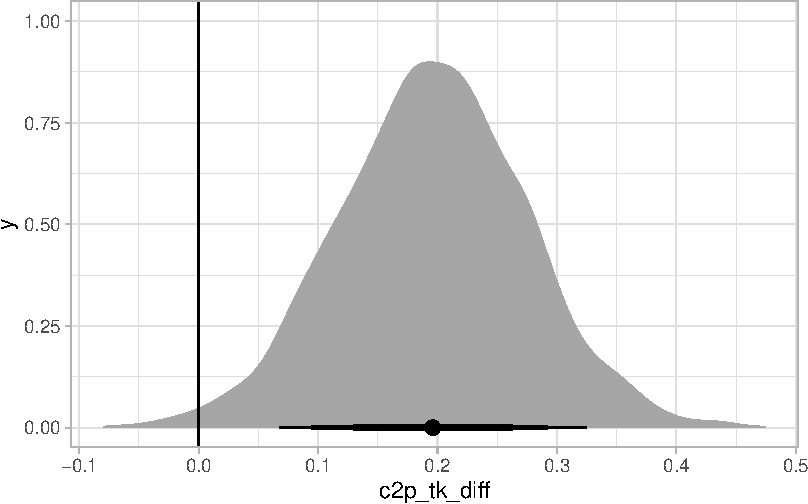
\includegraphics{manuscript_files/figure-pdf/fig-diff-p-tk-1.pdf}

}

\caption{\label{fig-diff-p-tk}}

\end{figure}%

Once we have the posterior difference, we can obtain CrIs of the
difference using \texttt{quantile2()} from the posterior package. Beware
that the values of the difference are in log-odds! We can convert these
into odd ratios with \texttt{exp()}.

\begin{Shaded}
\begin{Highlighting}[]
\FunctionTok{library}\NormalTok{(posterior)}
\end{Highlighting}
\end{Shaded}

\begin{verbatim}
This is posterior version 1.6.0
\end{verbatim}

\begin{verbatim}

Attaching package: 'posterior'
\end{verbatim}

\begin{verbatim}
The following objects are masked from 'package:stats':

    mad, sd, var
\end{verbatim}

\begin{verbatim}
The following objects are masked from 'package:base':

    %in%, match
\end{verbatim}

\begin{Shaded}
\begin{Highlighting}[]
\NormalTok{voi\_prop\_bm\_diff }\SpecialCharTok{|\textgreater{}} 
  \FunctionTok{reframe}\NormalTok{(}
    \CommentTok{\# 90\% CrI}
    \AttributeTok{q90 =} \FunctionTok{quantile2}\NormalTok{(c2p\_tk\_diff, }\AttributeTok{probs =} \FunctionTok{c}\NormalTok{(}\FloatTok{0.05}\NormalTok{, }\FloatTok{0.95}\NormalTok{)),}
    \CommentTok{\# 80\% CrI}
    \AttributeTok{q80 =} \FunctionTok{quantile2}\NormalTok{(c2p\_tk\_diff, }\AttributeTok{probs =} \FunctionTok{c}\NormalTok{(}\FloatTok{0.1}\NormalTok{, }\FloatTok{0.9}\NormalTok{)),}
    \CommentTok{\# 60\% CrI}
    \AttributeTok{q60 =} \FunctionTok{quantile2}\NormalTok{(c2p\_tk\_diff, }\AttributeTok{probs =} \FunctionTok{c}\NormalTok{(}\FloatTok{0.2}\NormalTok{, }\FloatTok{0.8}\NormalTok{)),}
\NormalTok{  ) }\SpecialCharTok{|\textgreater{}} 
  \CommentTok{\# exponentiate to get odd ratios and round to 2 digits}
  \FunctionTok{mutate}\NormalTok{(}\FunctionTok{across}\NormalTok{(}\FunctionTok{everything}\NormalTok{(), }\SpecialCharTok{\textasciitilde{}}\FunctionTok{round}\NormalTok{(}\FunctionTok{exp}\NormalTok{(.x), }\DecValTok{2}\NormalTok{)))}
\end{Highlighting}
\end{Shaded}

\begin{verbatim}
# A tibble: 2 x 3
    q90   q80   q60
  <dbl> <dbl> <dbl>
1  1.07  1.1   1.14
2  1.38  1.34  1.3 
\end{verbatim}

So, based on the model and data, there is a 90\% probability that the
voicing proportion in /p/ is 1.07-1.38 times longer (or 7-38\% increase)
than in /t, k/. At 80\% confidence, the change ratio is 1.10-1.34 (or
10-34\% increase) while at 60\% confidence is 1.14-1.30 (14-30\%
increase). In other words we can be quite confident that the voicing
proportion in /p/ is longer than in /t, k/ and that the increase is less
than 35\%.

brms comes with a convenient function, \texttt{conditional\_effects()},
to plot posterior means and CrIs based on predictors in the model. In
the following example, we plot the predicted proportion of voicing by
consonant and vowel.

\begin{Shaded}
\begin{Highlighting}[]
\FunctionTok{conditional\_effects}\NormalTok{(voi\_prop\_bm, }\StringTok{"c2:vowel"}\NormalTok{)}
\end{Highlighting}
\end{Shaded}

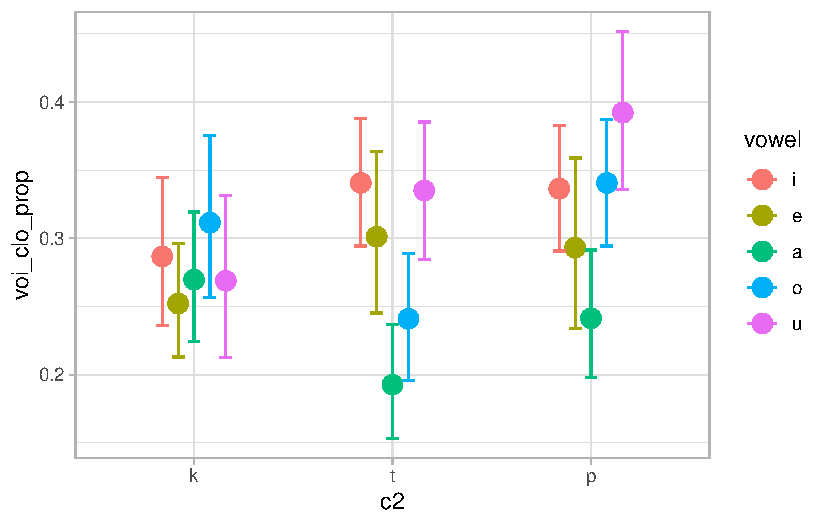
\includegraphics{manuscript_files/figure-pdf/voi-prop-bm-cond-1.pdf}

Finally, the package marginaleffects has two other convenience functions
that return CrIs of comparisons across predictor levels
(\texttt{avg\_comparisons()}) and CrIs of posterior predictions across
predictor levels (\texttt{avg\_predictions}). {[}XXX{]}

\begin{Shaded}
\begin{Highlighting}[]
\FunctionTok{library}\NormalTok{(marginaleffects)}

\FunctionTok{avg\_comparisons}\NormalTok{(voi\_prop\_bm, }\AttributeTok{variables =} \FunctionTok{list}\NormalTok{(}\AttributeTok{c2 =} \StringTok{"pairwise"}\NormalTok{), }\AttributeTok{conf\_level =} \FloatTok{0.8}\NormalTok{, }\AttributeTok{type =} \StringTok{"link"}\NormalTok{)}
\end{Highlighting}
\end{Shaded}

\begin{verbatim}

          Contrast Estimate   10.0 % 90.0 %
 mean(t) - mean(k)   0.0348 -0.00418 0.0738
 mean(p) - mean(k)   0.2176  0.17837 0.2558
 mean(p) - mean(t)   0.1829  0.14474 0.2192

Term: c2
Type:  link 
Columns: term, contrast, estimate, conf.low, conf.high, predicted_lo, predicted_hi, predicted, tmp_idx 
\end{verbatim}

\begin{Shaded}
\begin{Highlighting}[]
\FunctionTok{avg\_predictions}\NormalTok{(voi\_prop\_bm, }\AttributeTok{variables =} \StringTok{"vowel"}\NormalTok{, }\AttributeTok{conf\_level =} \FloatTok{0.8}\NormalTok{)}
\end{Highlighting}
\end{Shaded}

\begin{verbatim}

 vowel Estimate 10.0 % 90.0 %
     i    0.331  0.325  0.338
     e    0.300  0.293  0.307
     a    0.245  0.238  0.252
     o    0.305  0.298  0.312
     u    0.348  0.341  0.354

Type:  response 
Columns: vowel, estimate, conf.low, conf.high 
\end{verbatim}


\renewcommand\refname{Case study 2: pre-nasalisation in Greek}
  \bibliography{bibliography.bib}



\end{document}
